% Underlying graph for minimum spanning tree (mst) example
% Redrawn from Figure 5.3 of the textbook ``Algorithms'' by Dasgupta

\documentclass{standalone}

\usepackage{tikz}
\usetikzlibrary{calc, mindmap, positioning, backgrounds, fit}

\begin{document}
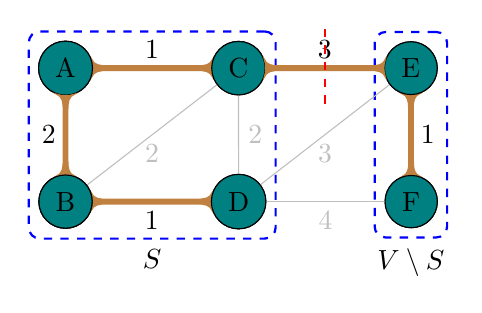
\begin{tikzpicture}[node distance = {1.0cm and 1.5cm}, 
  	v/.style = {draw, circle},
	e/.style = {gray!50},
  mstv/.style = {v, fill = teal},	% chosen by kruskal's algorithm
  mste/.style = {circle connection bar, brown, fill},
  cut/.style = {rectangle, rounded corners, dashed, draw, thick}	% cut
  ]
  \node (a) [v] {A};
  \node (c) [v, right = of a] {C};
  \node (e) [v, right = of c] {E};

  \draw (a) to node[above] {1} (c);
  \draw (c) to node[above] {3} (e);

  \node (b) [v, below = of a] {B};
  \node (d) [v, right = of b] {D};
  \node (f) [v, right = of d] {F};

  \draw (b) to node[below] {1} (d);
  \draw[e] (d) to node[below] {4} (f);

  \draw (a) to node[left] {2} (b);
  \draw[e] (c) to node[below] {2} (b);
  \draw[e] (c) to node[right] {2} (d);
  \draw[e] (e) to node[below] {3} (d);
  \draw (e) to node[right] {1} (f);

  % mst
  \draw[mste] (a) to (c); \node [mstv] at (a) {A}; \node [mstv] at (c) {C};
  \draw[mste] (b) to (d); \node [mstv] at (b) {B}; \node [mstv] at (d) {D};
  \draw[mste] (e) to (f); \node [mstv] at (e) {E}; \node [mstv] at (f) {F};
  \draw[mste] (a) to (b); \node [mstv] at (b) {B};
  \draw[mste] (c) to (e);

  % remove edge ce in mst
  \coordinate (cemid) at ($(c)!0.5!(e)$);
  \draw[red, dashed, thick] ($(cemid)+(0,0.5)$) to ($(cemid)-(0,0.5)$);

  \begin{pgfonlayer}{background}
	\node () [cut, blue, fit = (a) (b) (c) (d), label = {below:$S$}] {};
	\node () [cut, blue, fit = (e) (f), label = {below:$V \setminus S$}] {};
  \end{pgfonlayer}
  
\end{tikzpicture}
\end{document}